%%                                    %%
%% Generated from MathBook XML source %%
%%    on 2014-11-02T18:21:21-08:00    %%
%%                                    %%
\documentclass[10pt,]{article}
%
% Load geometry package to allow page margin adjustments
\usepackage{geometry}
\geometry{letterpaper,total={5.0in,9.0in}}
%% Custom entries to preamble, early

%% Page layout adjustment
\geometry{}
%%
%% Symbols, align environment, bracket-matrix
\usepackage{amsmath}
%% allow more columns to a matrix
%% can make this even bigger by overiding with preamble addition
\setcounter{MaxMatrixCols}{30}
\usepackage{amssymb}
%%
%% XML, MathJax Conflict Macros
%% Two nonstandard macros that MathJax supports automatically
%% so we always define them in order to allow their use and
%% maintain source level compatibility
%% This avoids using two XML entities in source mathematics
\newcommand{\lt}{<}
\newcommand{\gt}{>}
%%
%% Semantic Macros
%% To preserve meaning in a LaTeX file
%% Only defined here if required in this document
%% Environments with amsthm package
\usepackage{amsthm}
% Theorem-like enviroments, italicized statement, proof, etc
% Numbering: X.Y numbering scheme
%   i.e. Corollary 4.3 is third item in Chapter 4 of a book
%   i.e. Lemma 5.6 is sixth item in Section 5 of an article
\theoremstyle{plain}
\newtheorem{theorem}{Theorem}[section]
% Only variants actually used in document appear here
% Numbering: all theorem-like numbered consecutively
%   i.e. Corollary 4.3 follows Theorem 4.2
\newtheorem{corollary}[theorem]{Corollary}
% definition-like, normal text
\theoremstyle{definition}
\newtheorem{definition}{Definition}
\newtheorem{example}{Example}
\newtheorem{exercise}{Exercise}
%% Raster graphics inclusion, wrapped figures in paragraphs
\usepackage{graphicx}
%% Colors for Sage boxes and author tools (red hilites)
\usepackage[usenames,dvipsnames,svgnames,table]{xcolor}
%% Sage input, listings package: boxed, colored, line breaking
\usepackage{listings}
%% Tikz graphics
\usepackage{tikz}
\usetikzlibrary{backgrounds}
\usetikzlibrary{arrows,matrix}
%% Hyperlinking in PDFs, all links solid and blue
\usepackage[pdftex]{hyperref}
\hypersetup{colorlinks=true,linkcolor=blue,citecolor=blue,filecolor=blue,urlcolor=blue}
\hypersetup{pdftitle={Derivatives and Integrals}}
%%
%% Custom entries to preamble, late

%% Convenience macros

        \newcommand{\definiteintegral}[4]{\int_{#1}^{#2}\,#3\,d#4}
        \newcommand{\indefiniteintegral}[2]{\int#1\,d#2}
        
%% Title page information for article
\title{Derivatives and Integrals}
\author{Robert Beezer\\
Department of Mathematics and Computer Science\\
University of Puget Sound\newline Tacoma, Washington, USA\\
\href{mailto:beezer@pugetsound.edu}{\nolinkurl{beezer@pugetsound.edu}}
}
\date{November 2, 2014}
\begin{document}
%
\maketitle
%
\thispagestyle{empty}
%
\begin{abstract}
This is a sample of many of the things you can do with MathBook XML.  Sometimes the math makes sense, sometimes it seems to be written in the fist person, sort of like this Abstract.
%
\end{abstract}
%
Derivatives and Integrals\typeout{************************************************}
\typeout{Section 1 Introduction}
\typeout{************************************************}
%
\section{Introduction}\label{section-1}
%
We consider definite integrals of functions $f(x)$.  For example, \begin{displaymath}\definiteintegral{0}{2}{\sin^2(x)}{x}\end{displaymath}
%
\typeout{************************************************}
\typeout{Section 2 The Fundamental Theorem}
\typeout{************************************************}
%
\section{The Fundamental Theorem}\label{section-2}
%
There is a remarkable theorem:\footnote{And fortunately we do not need to try to write it in the margin!}
%
\begin{theorem}[The Fundamental Theorem of Calculus]\label{theorem-1}
If $f(x)$ is continuous, and the derivative of $F(x)$ is $f(x)$, then \begin{displaymath}\definiteintegral{a}{b}{f(x)}{x}=F(b)-F(a)\end{displaymath}
%
\end{theorem}
%
\begin{proof}
Left to the reader.
%
\end{proof}
%
\par You will find almost nothing about all this in the article \cite{bib-fundamental}, nor in the book \cite{bib-fcla}, since they belong in some other article, but we can cite them out-of-order for practice anyway.
%
\par When we are writing we do not always know what we want to cite, or just where subsequent material will end up.  For example, we might want a citation to $\langle\langle$some textbook about the FTC$\rangle\rangle$ or we might want to reference a later~$\langle\langle$chapter about DiffEq's$\rangle\rangle$.
%
\par We can also embed ``todo''s in the source, and selectively display them, so you may not see the one here in the output you are looking at now.  Or maybe you do see it?
%
\typeout{************************************************}
\typeout{Section 3 Computing Integrals}
\typeout{************************************************}
%
\section{Computing Integrals}\label{section-3}
%
Sage can compute definite integrals.  The output contains the approximate numerical value of the definite integral, followed by an upper bound  of the error in the approximation.
%
\begin{lstlisting}[language=Python,breaklines=true,breakatwhitespace=true,basicstyle=\small\ttfamily,columns=fixed,frame=single,frameround=tttt,backgroundcolor=\color{blue!10},xleftmargin=4ex,xrightmargin=4ex]
numerical_integral(sin(x)^2, (0, 2))
\end{lstlisting}
%
\begin{lstlisting}[language=Python,breaklines=true,breakatwhitespace=true,basicstyle=\small\ttfamily,columns=fixed,xleftmargin=8ex,xrightmargin=4ex]
(1.189200623826982, 1.320277913471315e-14)
\end{lstlisting}
%
\par Given the Fundamental Theorem, we would find the antiderivative useful.
%
\begin{lstlisting}[language=Python,breaklines=true,breakatwhitespace=true,basicstyle=\small\ttfamily,columns=fixed,frame=single,frameround=tttt,backgroundcolor=\color{blue!10},xleftmargin=4ex,xrightmargin=4ex]
integral(sin(x)^2, x)
\end{lstlisting}
%
\begin{lstlisting}[language=Python,breaklines=true,breakatwhitespace=true,basicstyle=\small\ttfamily,columns=fixed,xleftmargin=8ex,xrightmargin=4ex]
1/2*x - 1/4*sin(2*x)
\end{lstlisting}
%
\par The same command can be used to employ the antiderivative in the application of the Fundamental Theorem.  Notice that the answer is \emph{exact} and any further manipulation is likely to be simply producing a numerical approximation.
%
\begin{lstlisting}[language=Python,breaklines=true,breakatwhitespace=true,basicstyle=\small\ttfamily,columns=fixed,frame=single,frameround=tttt,backgroundcolor=\color{blue!10},xleftmargin=4ex,xrightmargin=4ex]
integral(sin(x)^2, (x, 0, 2))
\end{lstlisting}
%
\begin{lstlisting}[language=Python,breaklines=true,breakatwhitespace=true,basicstyle=\small\ttfamily,columns=fixed,xleftmargin=8ex,xrightmargin=4ex]
-1/4*sin(4) + 1
\end{lstlisting}
%
\typeout{************************************************}
\typeout{Section 4 An Interesting Corollary}
\typeout{************************************************}
%
\section{An Interesting Corollary}\label{section-4}
%
The Fundamental Theorem comes in two flavors, where usually one is a corollary of the other.
%
\begin{corollary}\label{corollary-1}
Suppose $f(x)$ is a continuous function.  Then \begin{displaymath}\frac{d}{dx}\definiteintegral{a}{x}{f(t)}{t}=f(x)\end{displaymath}
%
\end{corollary}
%
\begin{proof}
We simply take the indicated derivative, applying Theorem~\cref{theorem-FTC} at (\cref{equation-use-FTC}).
%
\begin{align}
\frac{d}{dx}\definiteintegral{a}{x}{f(t)}{t}&=\frac{d}{dx}\left(F(x)-F(a)\right)\label{equation-use-FTC}\\
&=\frac{d}{dx}F(x)-\frac{d}{dx}F(a)\notag\\
&=f(x)-0 = f(x)\label{}
\end{align}\end{proof}
%
\typeout{************************************************}
\typeout{Subsection 4.1 A Pedagogical Note}
\typeout{************************************************}
%
\subsection{A Pedagogical Note}\label{subsection-1}
%
The Fundamental Theorem explains why we use the same notation for a definite integral, which is a numerical calculation,\footnote{Which I think sometimes students lose sight of.} and an antiderivative, which is a symbolic expression.
%
\typeout{************************************************}
\typeout{Subsubsection 4.1.1 Advice}
\typeout{************************************************}
%
\subsubsection{Advice}\label{subsubsection-1}
%
Using an ``integral sign'' for an antiderivative (aka indefinite integral) would seem to make the Fundamental Theorem a \textit{fait accompli}.  So I would suggest not conflating the notation for two very different things until the Fundamental Theorem exposes them as being highly related.
%
\typeout{************************************************}
\typeout{Section 5 Some Facts and Figures}
\typeout{************************************************}
%
\section{Some Facts and Figures}\label{section-5}
%
Because of the Fundamental Theorem, for every derivative we know, there is an antiderivative we might find useful.  Because of the Fundamental Theorem of Calculus, we recycle the ``$\int$'' symbol as notation for an antiderivative.
%
\begin{itemize}
\item Derivatives\begin{enumerate}
\item $\frac{d}{dx}x^n = nx^{n-1}$%
\item $\frac{d}{dx}e^x = e^x$%
\item $\frac{d}{dx}\cos(x) = -\sin(x)$%
\end{enumerate}
%
%
\item Antiderivatives\begin{enumerate}
\item $\indefiniteintegral{x^n}{x} = \displaystyle\frac{x^{n-1}}{n+1}\text{ if }n\neq -1$%
\item $\indefiniteintegral{e^x}{x} = e^x$%
\item $\indefiniteintegral{\sin(x)}{x} = -\cos(x)$%
\end{enumerate}
%
%
\end{itemize}
%
\par You can gain a greater undestanding of derivatives by studying the graphs of functions with their derivatives.  Can you discern the derivative\textendash antiderivative relationship in Figure~\cref{figure-function-derivative}?
%
\begin{figure}[!htbp]
\centering
\includegraphics[width=350pt,]{images/cubic-function.png}\caption{A function and its derivative\label{figure-1}}
\end{figure}
%
\begin{figure}[!ht]
\centering
\includegraphics[width=350pt,]{images/cubic-function.png}\caption{testing the new float\label{figure-2}}
\end{figure}
%
\typeout{************************************************}
\typeout{Section 6 Some Advanced Ideas}
\typeout{************************************************}
%
\section{Some Advanced Ideas}\label{section-6}
%
The multi-row displayed mathematics in the proof of the Fundamental Theorem had equations aligned on the equals signs via the \& character.  Sometimes you don't want that.  Here is an example with some differential equations, with each equation centered and unnumbered,
            \begin{gather}
{\mathcal L}(y')(s) = s {\mathcal L}(y)(s) - y(0) = s Y(s) - y(0)\notag\\
{\mathcal L}(y'')(s) = s^2 {\mathcal L}(y)(s) - sy(0) - y'(0)= s^2 Y(s) - sy(0) - y'(0).\notag
\end{gather}
%
\par Table can get quite complex.  Simple ones are simpler, such as this example of numerical computations for Euler's method.
%
\begin{table}[thb]\centering
\label{table-1}\begin{tabular}{*{4}{c}}
\hline\hline $i$&$t_i$&$x_i$&$y_i$\\
\\\hline\hline 0&0&0&0.5000\\
1&0.20&0.1000&0.4800\\
2&0.40&0.1960&0.4560\\
3&0.60&0.2872&0.4295\\
4&0.80&0.3731&0.4027\\
5&1.00&0.4536&0.3783\\
6&1.20&0.5293&0.3591\\
7&1.40&0.6011&0.3480\\
8&1.60&0.6707&0.3474\\
9&1.80&0.7402&0.3603\\
10&2.00&0.8123&0.3900\\
\end{tabular}
\caption{Euler's approximation for Duffing's Equation with $h = 0.2$}
\end{table}
%
\typeout{************************************************}
\typeout{Section 7 Graphics}
\typeout{************************************************}
%
\section{Graphics}\label{section-7}
%
The Asymptote graphics language may be placed in your source to draw pictures.  For \LaTeX  processing you must have Asymptote's style file, \verb?asymptote.sty?, available, and then it is a three-step process: \LaTeX , \verb?asy?, \LaTeX .  For these reasons, the source is commented-out and you will see nothing below.  So you need to edit \verb?sample-article.tex? if you want to experiment.  Rules for formatting code are identical to those for Sage code.  For more on Asymptote and \LaTeX  see \url{http://asymptote.sourceforge.net/doc/LaTeX-usage.html}.
%
\par A simple Venn diagram example from the Asymptote documentation.
%
\typeout{************************************************}
\typeout{Section 8 Embedded Interactive Elements}
\typeout{************************************************}
%
\section{Embedded Interactive Elements}\label{section-8}
%
When outputting Web page versions, it is possible to embed a variety of dynamic interactive elements.  In a \LaTeX /PDF version, these will necessarily need to be replaced by some static substitute, such as a screenshot.
%
\typeout{************************************************}
\typeout{Subsection 8.1 GeoGebra}
\typeout{************************************************}
%
\subsection{GeoGebra}\label{subsection-2}
%
This first example of a  GeoGebra demonstration has just the controls for moving the three vertices on the circumfrence of the circle.  This is courtesy of Danny Parsons at the African Institute of Mathematical Sciences.  This demo requires Java, which could be problematic.
%
\par GeoGebra will create screenshots of demonstrations in tikz/\LaTeX  code.  For a static version, we use this as a figure.
%
\begin{figure}[!htbp]
\centering
\resizebox{0.75\textwidth}{!}{
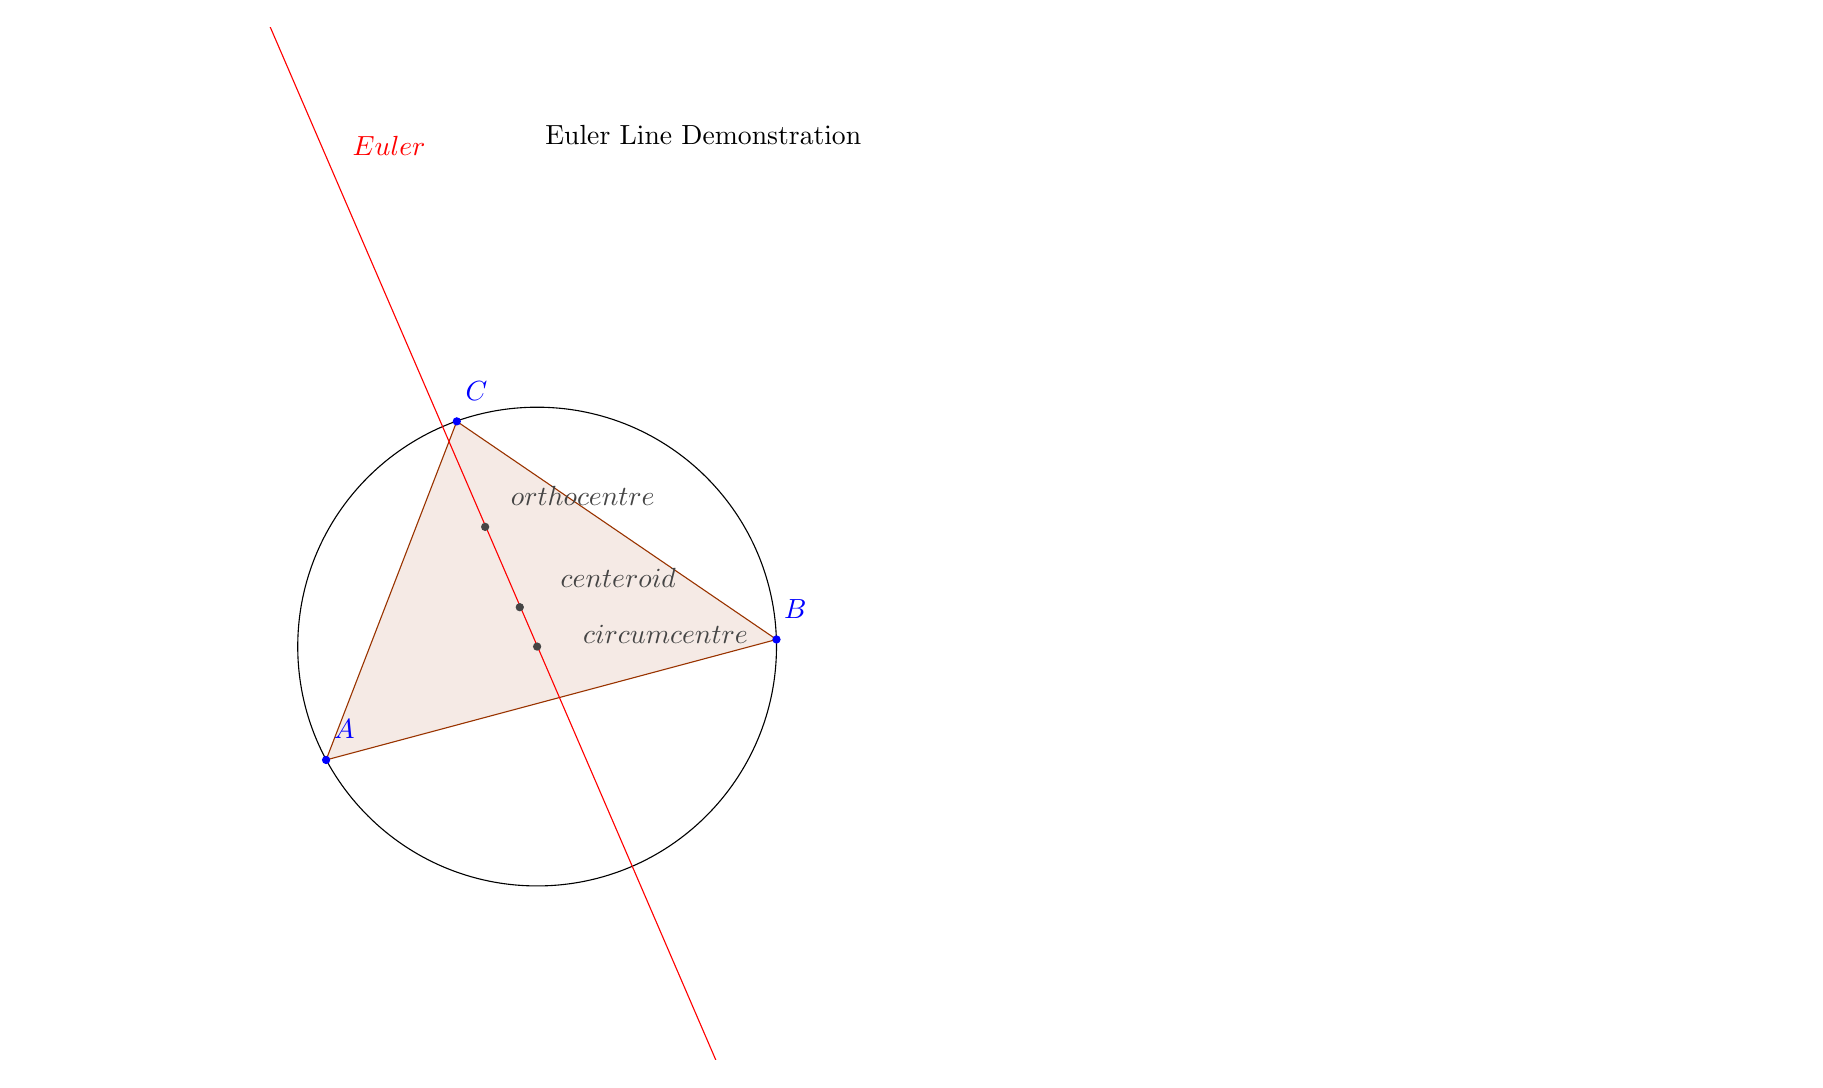
\begin{tikzpicture}

                            \definecolor{ffqqqq}{rgb}{1,0,0}
                            \definecolor{uuuuuu}{rgb}{0.27,0.27,0.27}
                            \definecolor{zzttqq}{rgb}{0.6,0.2,0}
                            \definecolor{qqqqff}{rgb}{0,0,1}
                            \clip(-8.34,-5.38) rectangle (14.1,7.73);
                            \fill[color=zzttqq,fill=zzttqq,fill opacity=0.1] (-4.55,-1.57) -- (1.17,-0.04) -- (-2.89,2.73) -- cycle;
                            \draw [color=zzttqq] (-4.55,-1.57)-- (1.17,-0.04);
                            \draw [color=zzttqq] (1.17,-0.04)-- (-2.89,2.73);
                            \draw [color=zzttqq] (-2.89,2.73)-- (-4.55,-1.57);
                            \draw(-1.87,-0.13) circle (3.04cm);
                            \draw [color=ffqqqq,domain=-8.34:14.1] plot(\x,{(-1.96-1.02*\x)/0.44});
                            \draw (-1.89,6.62) node[anchor=north west] {Euler Line Demonstration};
                            \fill [color=qqqqff] (-4.55,-1.57) circle (1.5pt);
                            \draw[color=qqqqff] (-4.32,-1.18) node {$A$};
                            \fill [color=qqqqff] (1.17,-0.04) circle (1.5pt);
                            \draw[color=qqqqff] (1.41,0.35) node {$B$};
                            \fill [color=qqqqff] (-2.89,2.73) circle (1.5pt);
                            \draw[color=qqqqff] (-2.64,3.11) node {$C$};
                            \fill [color=uuuuuu] (-2.09,0.37) circle (1.5pt);
                            \draw[color=uuuuuu] (-0.84,0.74) node {$centeroid$};
                            \fill [color=uuuuuu] (-1.87,-0.13) circle (1.5pt);
                            \draw[color=uuuuuu] (-0.24,0.02) node {$circumcentre$};
                            \fill [color=uuuuuu] (-2.53,1.39) circle (1.5pt);
                            \draw[color=uuuuuu] (-1.29,1.79) node {$orthocentre$};
                            \draw[color=ffqqqq] (-3.75,6.23) node {$Euler$};
                        \end{tikzpicture}
} % end box resizing
%
\caption{GeoGebra demonstration of the Euler Line\label{figure-3}}
\end{figure}
%
\par With a totally empty ``geogebra'' element, you will get a blank slate to play around in.   This is based on an example of embedding GeoGebra into Sage notebooks by Bruce Cohen.  Notice the full suite of menus and tools (in contrast to the previous example).
%
\par Again, this example will run with Java.  GeoGebra demonstrations can be run via HTML5 without invoking Java, but this seems to only be possible in the Chrome browser.  Support will be expanded, especially if requested.
%
\par\smallskip\centerline{Blank GeoGebra canvas is here in Web version.}\smallskip\typeout{************************************************}
\typeout{Section 9 Video}
\typeout{************************************************}
%
\section{Video}\label{section-9}
%
Embedded videos can make sense for a web version of your document. This is a video promoting the University of Puget Sound to potential new students.  Support is limited to WebM format initially, mp4 support will be easy to add.  This may require an HTML5 capable browser, such as Chrome, to render properly.
%
\begin{figure}[!htbp]
\centering
\caption{University of Puget Sound Promotional Video\label{figure-4}}
\end{figure}
%
\typeout{************************************************}
\typeout{Section 10 Exercises}
\typeout{************************************************}
%
\section{Exercises}\label{section-10}
%
\begin{exercise}\label{exercise-1}
Compute the definite integral $\definiteintegral{2}{4}{x^2}{x}$, not as an approximate value from a Riemann sum, but as an exact value based of the limit by using the Fundamental Theorem.
%
\par\smallskip\noindent\textbf{Solution.}\quad
An antiderivative of $x^2$ is $F(x)=x^3/3$, so by the FTC,\begin{displaymath}\definiteintegral{2}{4}{x^2}{x}=F(4)-F(2)=\frac{1}{3}\left(4^3-2^3\right)=\frac{56}{3}.\end{displaymath}
%
\end{exercise}
%
\begin{exercise}\label{exercise-2}
Can you prove Corollary~\cref{corollary-FTC-derivative} directly?
%
\end{exercise}
%
Generated: November 2, 2014, 18:21:21 (-08:00)
%
\begin{thebibliography}{99}
%
\bibitem{bib-judson-AATA}
Tom Judson, \textit{Abstract Algebra: Theory and Applications}, \textbf{55}
%
\bibitem{bib-fcla}
Robert A. Beezer, \textsl{A First Course in Linear Algebra},  (Congruent Press 2012).
%
\bibitem{bib-lay-book}
David C. Lay, \textsl{Linear Algebra and Its Applications},  (Pearson 2011).
%
\bibitem{bib-lay-article}
David C. Lay, ``Subspaces and Echelon Forms'', The College Mathematics Journal (January 1993),  (24) no. 1, 57-62.
%
\bibitem{bib-fundamental}
Gilbert Strang, ``The Fundamental Theorem of Linear Algebra'', The American Mathematical Monthly (November 1993),  (100) no. 9, 848-855.
%
\end{thebibliography}
%
\end{document}
